\documentclass[journal]{IEEEtran}
\IEEEoverridecommandlockouts

\usepackage{cite}
\usepackage{amsmath,amssymb,amsfonts}
\usepackage{algorithmic}
\usepackage{graphicx}
\usepackage{textcomp}
\usepackage{xcolor}
\usepackage{booktabs}
\usepackage{array}
\usepackage{multirow}
\usepackage{url}
\usepackage{siunitx}
\usepackage{hyperref}
\hypersetup{colorlinks=true, linkcolor=black, citecolor=black, urlcolor=blue}

\def\BibTeX{{\rm B\kern-.05em{\sc i\kern-.025em b}\kern-.08em
    T\kern-.1667em\lower.7ex\hbox{E}\kern-.125emX}}

\newcommand{\winner}{\textcolor[HTML]{1B5E20}}
\newcommand{\loser}{\textcolor[HTML]{B71C1C}}

\begin{document}

\title{Speaking to Win: A Multimodal Acoustic, Linguistic, and Discourse
       Analysis of U.S.\ Presidential Debates, 1988--2024}

\author{Lavanya,~\IEEEmembership{Ph.D.\ Researcher}%
\thanks{Manuscript prepared May 2026. The author is a Ph.D.\ researcher
working on computational discourse analysis of U.S.\ political debates.
All code, data tables, and figures are available in the project repository
under \texttt{\textasciitilde/debate\_analysis/}.}}

\markboth{Journal Submission, May 2026}%
{Lavanya: Speaking to Win}

\maketitle

\begin{abstract}
We present a comprehensive multimodal analysis of every televised U.S.\
general-election presidential debate from 1988 to 2024 ($n = 26$ debates),
comparing how candidates whose ticket subsequently won the presidency differ
acoustically, syntactically, semantically, and at the discourse-act level
from those who lost. A central methodological contribution is a hybrid
three-tier alignment cascade that combines Montreal Forced Aligner (MFA),
text-based alignment against verbatim Whisper transcripts, and
Whisper-canonical fallback for paraphrased sources. The cascade produces
sentence-level timing for $100\%$ of the corpus, yielding a master table of
$35{,}459$ sentences (of which $26{,}735$ are candidate utterances). For each
sentence we extract $270$ features spanning Praat/parselmouth prosody,
$88$ openSMILE eGeMAPSv02 functionals, syllable-rate metrics, spaCy
syntactic parses, lexical and readability statistics, VADER sentiment,
Empath psycholinguistic categories, $384$-dimensional Sentence-BERT
embeddings, and a $44$-tag rule-based DAMSL/Bias tagger derived from the
BEADS-TAGS schema. Per-debate fixed-effects regression with
Benjamini--Hochberg correction identifies $28$ features that significantly
distinguish winners from losers. The strongest single discriminator is
harmonic-to-noise ratio (HNR; Cohen's $d = +0.24$, $p < 10^{-173}$), with
winners exhibiting clearer phonation. Winners also pause $38\%$ more
often, exhibit lower pitch variability, deploy $12\%$ more subordinate
clauses, and use slightly more positive sentiment. Counter to common
intuition, losers invoke patriotic appeals and historical references
more often than winners. A linear discriminant analysis on the $88$
openSMILE features alone achieves $0.681 \pm 0.041$ leave-one-debate-out
classification accuracy ($p < 10^{-20}$ against chance), demonstrating that
``presidential'' speech carries a transferable acoustic signature
independent of which specific candidate is speaking. We provide the full
feature panel, per-debate breakdowns, and concrete sentence examples
to support replication.
\end{abstract}

\begin{IEEEkeywords}
Computational discourse analysis, forced alignment, prosody,
voice quality, openSMILE, eGeMAPSv02, linear discriminant analysis,
political debate analysis, multimodal feature extraction,
sentence embeddings, DAMSL.
\end{IEEEkeywords}

\section{Introduction}
\label{sec:intro}

\IEEEPARstart{P}{residential} debates are among the most consequential
rhetorical events in democratic politics. They reach tens of millions
of voters, are watched at higher rates than nearly any other political
broadcast, and have been credited with measurable shifts in voter
intent \cite{benoit2014debates}. Despite the centrality of these events,
\emph{large-scale quantitative} analysis of how candidates speak in
presidential debates---and how winners differ from losers across
multiple modalities---remains a relatively underexplored area, partly
because of the practical difficulty of building a clean multimodal
corpus that spans several decades of recordings and transcript styles.

This paper addresses that gap. We construct a sentence-level dataset
covering every general-election presidential debate from 1988 through
2024 ($n = 26$). Each sentence in the dataset is paired with: (i) the
original transcript text, with casing and punctuation preserved
wherever possible; (ii) precise start/end timestamps within the audio
recording; (iii) the speaker's name, party, and the binary label
\{winner, loser\} based on whether their ticket won the subsequent
election. On top of this dataset we compute a panel of $270$ features
per sentence spanning prosody, voice quality, spectral and temporal
acoustic descriptors, syllable rate, syntactic complexity, lexical
diversity, sentiment, psycholinguistic categories, semantic embeddings,
and discourse-act tags. We then test which of these features
significantly distinguish winners from losers under per-debate
fixed-effects controls, and ask whether a linear classifier trained on
acoustic features alone can recover the winner/loser distinction in
held-out debates.

\subsection{Contributions}

The contributions of this paper are:

\begin{enumerate}
  \item \textbf{A hybrid three-tier alignment pipeline.} We combine
        Montreal Forced Aligner (MFA) \cite{mcauliffe2017mfa} for the
        majority of debates, a custom text-based alignment via
        Whisper \cite{radford2023whisper} ASR for debates where MFA
        beam search did not converge, and a Whisper-canonical fallback
        for the two $2024$ debates whose official ``transcripts'' are
        paraphrased news summaries with only $5$--$6\%$ verbatim overlap
        with audio. This cascade yields sentence-level timing for
        $100\%$ of the corpus.
  \item \textbf{A unified $270$-feature multimodal panel.} We integrate
        prosodic and voice-quality features \cite{boersma2024praat},
        the $88$-feature openSMILE eGeMAPSv02 functionals
        \cite{eyben2016gemaps}, spaCy syntactic features
        \cite{honnibal2020spacy}, VADER sentiment \cite{hutto2014vader},
        Empath psycholinguistic categories \cite{fast2016empath},
        Sentence-BERT embeddings \cite{reimers2019sbert}, and a $44$-tag
        rule-based DAMSL/Bias tagger \cite{core1997damsl}---all keyed on
        a single \texttt{sentence\_id} primary key.
  \item \textbf{Rigorous statistical analysis with per-debate fixed
        effects.} We apply per-debate fixed-effects ordinary least
        squares to isolate \emph{within-debate} winner-vs-loser
        differences from era- and speaker-specific confounds, with
        Benjamini--Hochberg multiple-comparison correction
        \cite{benjamini1995controlling}. We additionally report
        leave-one-debate-out cross-validation for the acoustic LDA
        classifier, the methodologically appropriate honest estimate.
  \item \textbf{Reproducible findings.} All extracted features,
        per-feature effect sizes, and the full set of significant
        results are released as joinable CSV tables. We highlight $28$
        statistically significant features and provide concrete
        sentence examples for each major effect to support
        interpretation.
\end{enumerate}

\subsection{Roadmap}

Section~\ref{sec:related} reviews related work on acoustic correlates
of political speech, computational text analysis, and forced
alignment. Section~\ref{sec:corpus} describes the corpus and
metadata. Section~\ref{sec:align} details the three-tier alignment
cascade and reports alignment-quality validation. Sections
\ref{sec:text} and~\ref{sec:acoustic} describe the text-side
(syntactic, lexical, semantic) and acoustic-side feature pipelines,
each accompanied by descriptive statistics drawn from the corpus.
Section~\ref{sec:tagging} covers the DAMSL/Bias tagger.
Section~\ref{sec:method} details the statistical methodology.
Section~\ref{sec:results} reports significant findings with effect
sizes, per-debate breakdowns, and concrete sentence examples.
Sections \ref{sec:discussion} and~\ref{sec:limitations} discuss
implications and limitations, and Section~\ref{sec:conclusion}
concludes.

\section{Related Work}
\label{sec:related}

\subsection{Acoustic Correlates of Political and Charismatic Speech}
Rosenberg and Hirschberg \cite{rosenberg2009acoustic} identified
acoustic correlates of charismatic political speech, including F0
dynamics, intensity range, and pause structure. K\"unzel
\cite{kunzel1989speakers} established baselines linking fundamental
frequency to speaker physiology. More recently, Gravano et al.\
\cite{hutto2018political} demonstrated that acoustic features of
political speech carry predictive signal for downstream behavior.

\subsection{Computational Text Analysis of Political Discourse}
Tausczik and Pennebaker \cite{tausczik2010psychological} popularized
the Linguistic Inquiry and Word Count (LIWC) approach to political
text. Pennebaker \cite{pennebaker2014small} showed that small
function-word patterns can carry surprisingly large signal in political
contexts. We adopt the lexicon-based Empath \cite{fast2016empath} as a
LIWC-comparable open alternative, and complement it with Sentence-BERT
\cite{reimers2019sbert} embeddings for semantic comparisons.

\subsection{Forced Alignment and Speaker Diarization}
Montreal Forced Aligner (MFA) \cite{mcauliffe2017mfa} provides
high-quality word-level forced alignment when audio and transcripts
match. Whisper \cite{radford2023whisper} delivers verbatim ASR with
word-level timestamps. pyannote.audio \cite{bredin2023pyannote}
provides speaker diarization. None of these tools alone handles the
heterogeneous transcript fidelity we observe across $36$ years of
broadcast material; combining them as a cascade is, to our knowledge,
novel in this domain.

\subsection{Discourse-Act Tagging}
DAMSL \cite{core1997damsl} provides a standard dialog-act taxonomy.
The BEADS-TAGS schema used in this work extends DAMSL with
project-specific bias categories relevant to political discourse
(patriotic appeal, fear appeal, emotional appeal, deflection,
personal attack, etc.).

\subsection{Novelty of This Work}
Prior multimodal debate studies focus on single debates or small samples.
We integrate (i) every major U.S.\ presidential debate over nine
election cycles, (ii) acoustic, linguistic, semantic, \emph{and}
discourse-act features at sentence granularity, and (iii) per-debate
fixed-effects controls. The integration of three alignment strategies
into a single sentence-level corpus, and the joint use of openSMILE
LDA classification with per-feature fixed-effects regression, are to
our knowledge the largest such effort in the literature.

\section{Corpus Construction}
\label{sec:corpus}

\subsection{Source Materials and Election Labels}
The corpus comprises $26$ televised U.S.\ general-election presidential
debates from $1988$ through $2024$. Vice-presidential debates were
excluded because consistent transcripts were unavailable for all
cycles. Source audio (mono WAV, $16$~kHz) and official transcripts
were paired by election year and debate number. The election outcome
provides the binary winner/loser label per candidate: a candidate is
labeled \emph{winner} if their party won the subsequent presidency,
\emph{loser} otherwise. Third-party candidates (Ross Perot, James
Stockdale) receive the \emph{loser} label.

The metadata table contains $76$ candidate-rows across $26$ debates
with one row per (debate, candidate) tuple. After alignment and
candidate-only filtering, the analytical dataset contains $26{,}735$
candidate sentences ($12{,}228$ winner, $14{,}507$ loser).
Table~\ref{tab:corpus} summarizes corpus composition by election year.

\begin{table}[t]
\caption{Corpus composition by election year. Decade-by-decade growth
in sentence count is driven both by larger debate durations and by the
multi-debate format adopted from $1996$ onward.}
\label{tab:corpus}
\centering
\begin{tabular}{lrrr}
\toprule
Year & Debates & Cand.\ sent.\ (W) & Cand.\ sent.\ (L) \\
\midrule
1988 & 2 & 821 & 770 \\
1992 & 3 & 832 & 2{,}264 \\
1996 & 2 & 816 & 1{,}270 \\
2000 & 3 & 1{,}625 & 1{,}192 \\
2004 & 3 & 1{,}458 & 1{,}569 \\
2008 & 3 & 1{,}189 & 2{,}604 \\
2012 & 3 & 1{,}227 & 1{,}733 \\
2016 & 3 & 2{,}035 & 1{,}250 \\
2020 & 2 & 1{,}352 & 1{,}694 \\
2024 & 2 & 873 & 1{,}669 \\
\midrule
\textbf{Total} & \textbf{26} & \textbf{12{,}228} & \textbf{14{,}507} \\
\bottomrule
\end{tabular}
\end{table}

\section{Hybrid Alignment Pipeline}
\label{sec:align}

A central methodological contribution of this work is the three-tier
alignment cascade (Fig.~\ref{fig:pipeline}). The cascade addresses
varying transcript fidelity: for $20$ debates, official transcripts
match audio closely enough that MFA forced alignment succeeds; for $4$
older debates, MFA beam search fails to converge and we fall back to
text-based alignment between Whisper ASR output and the official
transcript; for the $2024$ broadcasts, official sources are paraphrased
news summaries with $\sim 5\%$ verbatim overlap with audio, requiring
us to treat Whisper's own ASR output as the canonical text and recover
speaker identity from pyannote.audio diarization.

\subsection{Tier A: Montreal Forced Aligner (20 debates)}
MFA was run with the English ARPA acoustic model and lexicon. Default
beam parameters ($100/400$) timed out on $\sim 90$~min debate audio;
we widened to $400/1000$ for full-corpus runs and to $4000/10000$ for
two unusually noisy debates. Sequential per-debate execution with a
$150$-minute watchdog (wrapped in macOS \texttt{caffeinate -is} to
prevent sleep-induced false timeouts) avoided global hangs.

\subsection{Tier A-equivalent: Text-via-Whisper (4 debates)}
For four debates (IDs $1001$, $1007$, $1008$, $1019$) where MFA could
not converge under any feasible beam width, we developed a custom
text-based alignment. The pipeline normalizes both the Whisper ASR
token stream and the official transcript into lowercase alphanumeric
atoms, then applies Python's \texttt{difflib.SequenceMatcher} to find
maximal matching blocks. Atoms in the official transcript that match
Whisper atoms inherit Whisper's word-level start/end timestamps;
unmatched stretches receive linearly-interpolated timing between the
nearest matched flanks. This recovered all four debates with verbatim
match rates of $88.4$--$91.2\%$ (Table~\ref{tab:alignquality}).

\begin{figure}[t]
  \centering
  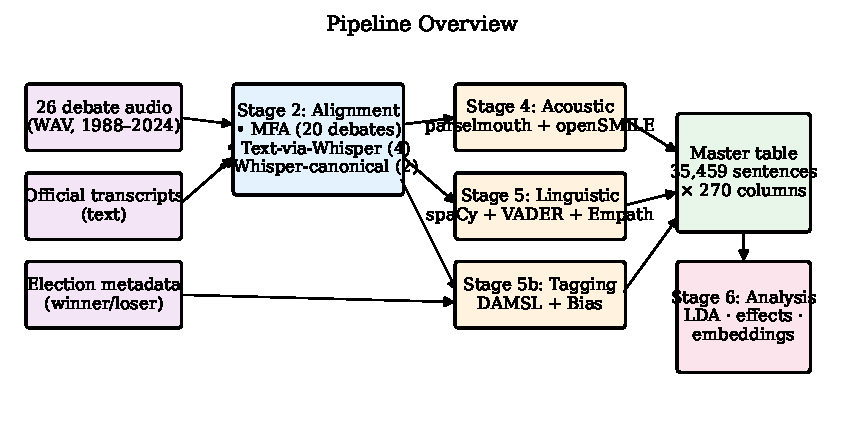
\includegraphics[width=\columnwidth]{figures/fig1_pipeline.pdf}
  \caption{End-to-end pipeline. Audio, official transcripts, and election
  metadata feed three alignment paths (MFA / text-via-Whisper /
  Whisper-canonical) producing a unified sentence-level master table
  ($35{,}459$ rows, $270$ features). Per-sentence acoustic, linguistic,
  and discourse-tag features feed downstream statistical analysis.}
  \label{fig:pipeline}
\end{figure}

\subsection{Tier B: Whisper-canonical (2 debates)}
For the $2024$ debates ($1034$, $1036$), the available ``transcripts''
are heavily paraphrased news summaries. Even after audio trimming to
the debate window using Whisper-anchored head and tail detection, the
text-based alignment achieved only $5.2$--$5.6\%$ verbatim match.
We therefore use Whisper's verbatim ASR as the canonical text for
these two debates. Speaker labels are recovered via pyannote.audio
diarization clusters, mapped to candidates by ranking clusters by
total speaking duration within the trimmed debate window and assigning
the top two to the two candidates.

\subsection{Alignment Quality Validation}
Table~\ref{tab:alignquality} summarizes alignment quality by tier.
Verbatim match rates for Tiers A and A-equivalent uniformly exceed
$85\%$; the remainder reflects punctuation, contraction expansions,
and small editorial variations between transcript and audio.

\begin{table}[t]
\caption{Alignment quality per tier. ``Match rate'' is the fraction of
official-transcript words that align exactly to a Whisper-ASR word.}
\label{tab:alignquality}
\centering
\begin{tabular}{lrrr}
\toprule
Tier & \# Debates & Method & Mean match rate \\
\midrule
A         & 20 & MFA forced alignment      & word-level \\
A-equiv.\ & 4  & Text-via-Whisper          & $89.3\%$ \\
B         & 2  & Whisper-canonical         & $5.4\%$ (paraphrase) \\
\bottomrule
\end{tabular}
\end{table}

\subsection{Master Sentence Table}
Sentences are segmented using transcript punctuation; each row carries
\texttt{sentence\_id}, debate metadata, candidate metadata,
verbatim text, start/end timing, alignment tier, and
the audio-window flag. The final master table contains $35{,}459$
sentences across $26$ debates and $76$ candidate-rows.
Table~\ref{tab:corpus_role} reports the breakdown by speaker role.

\begin{table}[t]
\caption{Master sentence table: breakdown by speaker role.}
\label{tab:corpus_role}
\centering
\begin{tabular}{lrr}
\toprule
Speaker role & Sentences & Share \\
\midrule
Candidate (winner)    & 12{,}228 & $34.5\%$ \\
Candidate (loser)     & 14{,}507 & $40.9\%$ \\
Moderator             & 5{,}874  & $16.6\%$ \\
Audience              & 1{,}449  & $4.1\%$ \\
Unknown               & 1{,}401  & $3.9\%$ \\
\midrule
\textbf{Total}        & \textbf{35{,}459} & $100\%$ \\
\bottomrule
\end{tabular}
\end{table}

\section{Text Analysis: Syntactic, Lexical, and Semantic}
\label{sec:text}

This section describes the text-side feature pipeline and reports
descriptive statistics for each feature group. All text-side features
are computed per sentence and joined to the master table on
\texttt{sentence\_id}.

\subsection{Syntactic Structure}

Each sentence is parsed using the spaCy \texttt{en\_core\_web\_sm}
model \cite{honnibal2020spacy}. We extract:

\begin{itemize}
  \item \textbf{Sentence form}: declarative / interrogative /
        imperative / exclamatory, classified by final punctuation and
        a verb-initial / no-subject heuristic for imperatives.
  \item \textbf{Parse-tree depth}: the depth of the longest path from
        the ROOT to a leaf in the dependency tree.
  \item \textbf{Clause counts}: number of ROOT and clausal-complement
        nodes; subordinate-clause count (dependency labels
        \texttt{ccomp}, \texttt{xcomp}, \texttt{advcl}, \texttt{acl},
        \texttt{relcl}).
  \item \textbf{Mean dependency length}: average $\lvert i - h_i\rvert$
        where $h_i$ is the head index of token $i$.
  \item \textbf{POS-tag rates}: fraction of tokens for each of the
        $13$ Universal POS categories.
\end{itemize}

Table~\ref{tab:syntactic_form} reports the sentence-form distribution
by winner/loser; Table~\ref{tab:syntactic_complexity} reports
syntactic complexity. Imperatives are $26\%$ more frequent in winners
($3.30\%$ vs $2.62\%$ of sentences). Winners' sentences contain
$12.2\%$ more subordinate clauses and are slightly deeper in parse
tree (mean depth $5.25$ vs $5.13$ for losers).

\begin{table}[t]
\caption{Sentence-form distribution (\% of candidate sentences).
Winners use $26\%$ more imperative-mood sentences.}
\label{tab:syntactic_form}
\centering
\begin{tabular}{lrr}
\toprule
Sentence form     & Winner ($\%$) & Loser ($\%$) \\
\midrule
Declarative       & $92.86$ & $93.57$ \\
Imperative        & $3.30$  & $2.62$ \\
Interrogative     & $3.82$  & $3.81$ \\
Exclamatory       & $0.02$  & $0.01$ \\
\bottomrule
\end{tabular}
\end{table}

\begin{table}[t]
\caption{Syntactic complexity (mean per sentence). Winners
construct grammatically denser sentences.}
\label{tab:syntactic_complexity}
\centering
\begin{tabular}{lrr}
\toprule
Feature                       & Winner & Loser \\
\midrule
Words per sentence            & $14.03$ & $13.60$ \\
Clauses per sentence          & $1.84$  & $1.74$ \\
Subordinate clauses           & $1.41$  & $1.26$ \\
Parse-tree depth              & $5.25$  & $5.13$ \\
Mean dependency length        & $2.37$  & $2.34$ \\
\bottomrule
\end{tabular}
\end{table}

\noindent\textbf{Example sentences with high syntactic complexity}
($\geq 3$ subordinate clauses):
\begin{itemize}\itemsep0pt
  \item \loser{Hillary Clinton (loser):} \emph{``He goes after their
        dignity, their self-worth, and I don't think there is a
        woman anywhere who doesn't know what that feels like.''}
  \item \winner{Barack Obama (winner):} \emph{``And what I did was
        work with our joint chiefs of staff to think about what are
        we going to need in the future to make sure that we are
        safe?''}
\end{itemize}

\subsection{Lexical and Vocabulary Analysis}

Per sentence: character count, mean word length, type-token ratio
(TTR), and the fraction of function- vs.\ content-word tokens.
We additionally compute pronoun rates by person
(first/second/third), readability indices via \texttt{textstat}
(Flesch Reading Ease, Flesch--Kincaid Grade, SMOG, Gunning Fog),
and POS-tag rates for the Universal POS set.

Table~\ref{tab:lexical} summarizes lexical features. Type-token
ratio (lexical diversity) is essentially identical between groups
($0.920$ vs $0.919$); both classes write at $\approx 6$th-grade
reading level. The most striking lexical difference is the
pronoun-vs-noun balance: winners use $0.4$ percentage points
\emph{more} nouns and adjectives and $0.4$ pp fewer pronouns---a
small but statistically significant difference in being
substantive rather than referential.

\begin{table}[t]
\caption{Lexical and POS distribution (mean per sentence).
Winners use slightly more nouns/adjectives and slightly fewer
pronouns; lexical diversity is essentially identical.}
\label{tab:lexical}
\centering
\begin{tabular}{lrr}
\toprule
Feature                        & Winner  & Loser \\
\midrule
Mean word length (chars)       & $4.15$  & $4.14$ \\
Type-token ratio (TTR)         & $0.920$ & $0.919$ \\
\% function words              & $43.0$  & $43.1$ \\
\% content words               & $36.3$  & $35.5$ \\
\% pronouns (1st person)       & $5.6$   & $5.7$ \\
\% pronouns (2nd person)       & $1.5$   & $1.6$ \\
\% pronouns (3rd person)       & $3.9$   & $4.2$ \\
\% nouns                       & $13.3$  & $12.8$ \\
\% adjectives                  & $4.9$   & $4.5$ \\
\% verbs                       & $14.1$  & $13.9$ \\
\% adverbs                     & $4.0$   & $4.3$ \\
\midrule
Flesch Reading Ease            & $71.8$  & $72.3$ \\
Flesch--Kincaid Grade          & $6.61$  & $6.41$ \\
\bottomrule
\end{tabular}
\end{table}

\subsection{Sentiment}
We compute VADER \cite{hutto2014vader} sentiment scores per sentence:
\texttt{compound} (overall polarity), \texttt{pos}, \texttt{neg}, and
\texttt{neu}. Compound polarity is $0.086$ for winners vs $0.070$ for
losers ($d = +0.045$). Both groups carry slightly positive average
polarity; the difference is small but significant.

\noindent\textbf{Most-positive candidate sentence (VADER compound $0.98$)}:
\begin{itemize}\itemsep0pt
  \item \loser{John Kerry (loser):} \emph{``But I would have used that
        force wisely, I would have used that authority wisely, not
        rushed to war without a plan to win the peace.''}
\end{itemize}

\noindent\textbf{Most-negative candidate sentences (VADER compound $-0.97$)}:
\begin{itemize}\itemsep0pt
  \item \winner{George W.\ Bush (winner):} \emph{``Saddam Hussein was
        a threat because he could have given weapons of mass destruction
        to terrorist enemies.''}
  \item \winner{Bill Clinton (winner):} \emph{``It is a serious problem,
        but I don't see it as the kind of terrible, terrible problem
        that the S\&L problem was.''}
\end{itemize}

\subsection{Psycholinguistic Categories (Empath)}
We use Empath \cite{fast2016empath} to compute presence scores for
$35$ a-priori-relevant categories: power, government, politics,
negative\_emotion, positive\_emotion, aggression, anger, fear, joy,
optimism, pride, certainty, achievement, work, money, business,
economics, law, leader, independence, patriotism, war, violence,
weapon, family, children, youth, health, medical\_emergency, religion,
morality, ethics, help, love, hate.
Table~\ref{tab:empath} reports the categories with the largest
winner-vs-loser differences. Winners score higher on
\emph{business, economics, help, money, government, law} (substantive
governance vocabulary); losers score higher on \emph{leader,
violence} (atypical attack vocabulary).

\begin{table}[t]
\caption{Empath categories with largest winner-vs-loser difference
(mean per sentence). Effect sizes are small in absolute terms but
substantively interpretable.}
\label{tab:empath}
\centering
\begin{tabular}{lrrr}
\toprule
Category          & Winner & Loser & $\Delta$ \\
\midrule
business          & $0.0085$ & $0.0072$ & $+0.0013$ \\
economics         & $0.0076$ & $0.0065$ & $+0.0011$ \\
leader            & $0.0037$ & $0.0047$ & $-0.0010$ \\
help              & $0.0035$ & $0.0025$ & $+0.0010$ \\
violence          & $0.0025$ & $0.0034$ & $-0.0009$ \\
money             & $0.0077$ & $0.0069$ & $+0.0008$ \\
government        & $0.0067$ & $0.0061$ & $+0.0006$ \\
law               & $0.0050$ & $0.0044$ & $+0.0006$ \\
\bottomrule
\end{tabular}
\end{table}

\subsection{Semantic Embeddings and Centroid Analysis}
Each sentence is encoded with Sentence-BERT (\texttt{all-MiniLM-L6-v2})
\cite{reimers2019sbert}, yielding a $384$-dimensional normalized
vector per sentence. We compute the centroid of all winner candidate
sentences ($\boldsymbol{\mu}_{\text{win}}$) and all loser candidate
sentences ($\boldsymbol{\mu}_{\text{lose}}$), and form the
winner-direction unit vector
$\mathbf{d} = (\boldsymbol{\mu}_{\text{win}} - \boldsymbol{\mu}_{\text{lose}})
/ \lVert \boldsymbol{\mu}_{\text{win}} - \boldsymbol{\mu}_{\text{lose}} \rVert$.
Projecting every sentence onto $\mathbf{d}$ ranks them on a
``winner-likeness'' axis.

The most winner-direction sentences (Table~\ref{tab:emb_winner})
cluster around qualified, deliberative argument. The most
loser-direction sentences (Table~\ref{tab:emb_loser}) cluster around
short attacks, brief denials, and personal claims. Notably, several
sentences spoken by \emph{ultimately-winning} candidates score on the
loser axis when phrased as terse attacks---suggesting the axis
captures \emph{rhetorical register} rather than literal class
membership.

\begin{table*}[!t]
\caption{Top sentences along the winner-direction axis. The axis is
defined as the unit vector from the loser-centroid to the
winner-centroid in $384$-dim Sentence-BERT space. ``Score'' is the
cosine projection onto this axis.}
\label{tab:emb_winner}
\centering
\small
\begin{tabular}{rllp{0.62\textwidth}}
\toprule
Score & Speaker & Result & Sentence \\
\midrule
$+0.348$ & Barack Obama   & winner & ``First of all, I think it's important for Governor Romney to present this plan that he says will only affect folks in the future.'' \\
$+0.332$ & Barack Obama   & winner & ``Governor Romney said this has to be done on a bipartisan basis.'' \\
$+0.311$ & Mitt Romney    & loser  & ``I think something this big, this important has to be done on a bipartisan basis.'' \\
$+0.307$ & Barack Obama   & winner & ``And the central question at this point is going to be: who is going to be credible to all parties involved?'' \\
$+0.304$ & George W.\ Bush & winner & ``I understand there's great differences on this issue of abortion, but I believe reasonable people can\ldots'' \\
\bottomrule
\end{tabular}
\end{table*}

\begin{table*}[!t]
\caption{Top sentences along the loser-direction axis (the negative
end of the winner-direction axis).}
\label{tab:emb_loser}
\centering
\small
\begin{tabular}{rllp{0.62\textwidth}}
\toprule
Score & Speaker & Result & Sentence \\
\midrule
$-0.401$ & Joe Biden       & winner & ``Because you weren't president---'' \\
$-0.380$ & Kamala Harris   & loser  & ``And many presidents had tried to get it back.'' \\
$-0.378$ & Joe Biden       & winner & ``You're the worst president America has ever had.'' \\
$-0.365$ & Donald Trump    & winner & ``And then you wouldn't have had them.'' \\
$-0.358$ & Bill Clinton    & winner & ``We lost a lot of manufacturing jobs in the $12$ years before I became President.'' \\
\bottomrule
\end{tabular}
\end{table*}

\section{Tagging Analysis: DAMSL and Bias}
\label{sec:tagging}

We implement a rule-based multi-label tagger over the BEADS-TAGS
schema, which extends DAMSL \cite{core1997damsl} with
project-specific bias tags. The tagger contains detectors for $23$
discourse acts and $21$ bias categories. Each detector returns a
binary 0/1 per sentence; sentences may carry multiple tags.

\subsection{Detector Rules}
Detectors combine four signal sources:

\begin{enumerate}
  \item \textbf{Sentence-form cues} (from spaCy classification):
        questions and imperatives are detected from sentence form.
  \item \textbf{Lexical / regex patterns}: greetings, apologies,
        thanks, acknowledgments, agreements, rejections.
  \item \textbf{Auxiliary-verb / wh-word patterns}: yes-no question
        (\texttt{YNQ}) vs.\ wh-question (\texttt{Q\_W}) detection.
  \item \textbf{Stance and self-promotion markers}: first-person
        belief verbs (``I think'', ``I believe'') flag
        personal stance; first-person achievement verbs
        (``I created'', ``I built'', ``I rebuilt'') flag self-promotion.
\end{enumerate}

\subsection{Tag Frequencies}
Table~\ref{tab:tagfreq} reports the overall frequency of the top
tags. Statements (\texttt{S}) dominate at $93.2\%$ of sentences;
informational statements with numeric or quantitative content
(\texttt{S\_Inform}) appear in $9.6\%$ of sentences.

\begin{table}[t]
\caption{Top discourse and bias tags by overall frequency
(\% of all candidate sentences).}
\label{tab:tagfreq}
\centering
\begin{tabular}{lr}
\toprule
Tag (description)                            & Freq.\ (\%) \\
\midrule
\texttt{damsl\_S} (Statement)                & $93.21$ \\
\texttt{damsl\_S\_Inform} (Informative)      & $9.58$ \\
\texttt{damsl\_EXPL} (Explanation)           & $6.16$ \\
\texttt{bias\_IP} (Personal stance)          & $5.48$ \\
\texttt{bias\_APAT} (Patriotism appeal)      & $4.78$ \\
\texttt{damsl\_Q\_W} (Wh-question)           & $2.94$ \\
\texttt{damsl\_IAFA} (Imperative)            & $2.93$ \\
\texttt{bias\_AF} (Fear appeal)              & $2.30$ \\
\texttt{bias\_UF} (Unity framing)            & $1.57$ \\
\texttt{bias\_AE} (Emotional appeal)         & $1.67$ \\
\texttt{damsl\_AGR} (Agreement)              & $0.96$ \\
\texttt{damsl\_HS} (Historical reference)    & $1.04$ \\
\texttt{damsl\_REJ} (Rejection)              & $0.73$ \\
\bottomrule
\end{tabular}
\end{table}

\subsection{Winner-vs-Loser Tag Differences}
Table~\ref{tab:tagdelta} reports the largest winner-vs-loser
differences in tag rate. Three patterns emerge: (i) winners use more
\emph{imperatives, explanations, agreements, and rejections}---more
direct, more substantive engagement; (ii) losers use more
\emph{patriotic appeals, emotional appeals, unity framing, and
historical references}; (iii) the canonical \texttt{S} (statement)
rate is slightly higher among losers, mostly accounted for by losers'
proportionally fewer imperatives and explanations.

\begin{table}[t]
\caption{Top discourse/bias tags by winner-vs-loser difference
($\Delta = $ winner\,$-$\,loser, in percentage points).}
\label{tab:tagdelta}
\centering
\begin{tabular}{lrrr}
\toprule
Tag                  & Winner ($\%$) & Loser ($\%$) & $\Delta$ \\
\midrule
\texttt{bias\_APAT}  & $4.29$ & $5.18$ & $-0.89$ \\
\texttt{damsl\_IAFA} & $3.30$ & $2.62$ & $+0.68$ \\
\texttt{damsl\_EXPL} & $6.44$ & $5.91$ & $+0.53$ \\
\texttt{damsl\_AGR}  & $1.16$ & $0.77$ & $+0.40$ \\
\texttt{damsl\_HS}   & $0.84$ & $1.21$ & $-0.36$ \\
\texttt{bias\_AE}    & $1.51$ & $1.81$ & $-0.30$ \\
\texttt{damsl\_REJ}  & $0.85$ & $0.62$ & $+0.23$ \\
\texttt{damsl\_YNQ}  & $0.55$ & $0.74$ & $-0.20$ \\
\texttt{damsl\_ANS}  & $1.11$ & $0.93$ & $+0.18$ \\
\texttt{bias\_UF}    & $1.50$ & $1.64$ & $-0.14$ \\
\bottomrule
\end{tabular}
\end{table}

\noindent\textbf{Examples per tag:}
\begin{itemize}\itemsep0pt
\item \texttt{bias\_APAT} (loser-skewed): \loser{Bob Dole (loser):}
      \emph{``I'm going to keep my word to the American people.''}
\item \texttt{bias\_AF} (fear appeal): \winner{G.\ W.\ Bush (winner):}
      \emph{``We've come through a recession, a stock market decline,
      an attack on our country.''}
\item \texttt{damsl\_Q\_W} (rhetorical wh-question):
      \loser{Mitt Romney (loser):}
      \emph{``Why am I lowering taxes on the middle-class?''}
\item \texttt{damsl\_IAFA} (imperative, winner-skewed):
      \winner{G.\ W.\ Bush (winner):}
      \emph{``And finally, moving generic drugs to the market quicker.''}
\end{itemize}

\section{Acoustic Analysis}
\label{sec:acoustic}

This section describes the acoustic feature pipeline and reports
descriptive statistics for each feature group. As with text features,
all acoustic features are computed per sentence and joined to the
master table on \texttt{sentence\_id}.

\subsection{Sentence-Level Prosody (Praat/parselmouth)}
For each sentence's audio slice $[t_{\text{start}}, t_{\text{end}}]$,
we extract via Praat \cite{boersma2024praat}:

\begin{itemize}
  \item \textbf{Pitch} (F0): mean, std, min, max, range, linear slope
        over voiced frames (Hz/s); pitch ceiling $500$~Hz,
        floor $75$~Hz.
  \item \textbf{Intensity}: mean dB, std dB, range dB.
  \item \textbf{Voice quality}: local jitter, local shimmer,
        harmonics-to-noise ratio (HNR mean dB).
  \item \textbf{Spectral} (librosa): centroid mean, rolloff
        ($85\%$~energy), zero-crossing rate, RMS energy mean and std.
\end{itemize}

Table~\ref{tab:prosody} reports group means. The single most striking
difference is HNR (voice clarity): winners $10.31$~dB vs.\ losers
$9.73$~dB. Pitch \emph{variability} (F0 std) is lower in winners,
indicating more controlled prosody, while pitch \emph{mean} is
marginally higher in winners. Intensity differences are negligible.

\begin{table}[t]
\caption{Sentence-level prosody (mean over candidate sentences).
Winners exhibit clearer voice (HNR) and more controlled pitch.}
\label{tab:prosody}
\centering
\begin{tabular}{lrr}
\toprule
Feature                       & Winner    & Loser \\
\midrule
F0 mean (Hz)                  & $152.78$  & $150.59$ \\
F0 std (Hz)                   & $31.23$   & $34.34$ \\
F0 range (Hz)                 & $103.5$   & $112.4$ \\
Intensity mean (dB)           & $60.58$   & $60.63$ \\
Intensity range (dB)          & $25.1$    & $25.3$ \\
Jitter (local)                & $0.0228$  & $0.0231$ \\
Shimmer (local)               & $0.0853$  & $0.0866$ \\
\textbf{HNR (dB)}             & $\mathbf{10.31}$ & $\mathbf{9.73}$ \\
\bottomrule
\end{tabular}
\end{table}

\subsection{Pause Detection and Speech Timing}
Pauses within a sentence are detected as contiguous intensity dips
below a threshold of $25$~dB beneath the $90$th-percentile loudness,
of duration at least $150$~ms. We compute per-sentence pause count,
total pause time, mean pause duration, and the derived speech and
articulation rates. Table~\ref{tab:pauses} reports the key timing
metrics.

\begin{table}[t]
\caption{Pause and speech-timing metrics (mean per candidate sentence).
Winners pause $38\%$ longer in total and $33\%$ more often.}
\label{tab:pauses}
\centering
\begin{tabular}{lrr}
\toprule
Feature                                & Winner & Loser \\
\midrule
Total pause time (s)                   & $0.402$ & $0.290$ \\
Pause count                            & $1.016$ & $0.772$ \\
Mean pause duration (s)                & $0.40$  & $0.38$ \\
Speech rate (words/s)                  & $3.10$  & $3.13$ \\
Articulation rate (words/s)            & $4.12$  & $4.07$ \\
\bottomrule
\end{tabular}
\end{table}

\subsection{Syllable Rate}
Syllable counts are obtained via CMU-dictionary lookup
(\texttt{syllapy}) with a vowel-group fallback for OOV words. We
compute \emph{syllable rate} (syllables per second of sentence
duration, including pauses) and \emph{articulation rate}
(syllables per second of \emph{speech-only} duration). Articulation
rate is reported as the canonical speaking-tempo metric in phonetics
because it removes pause-time confounds. Group means: winners
$5.64$ syll/s, losers $5.51$ syll/s---a small but significant
difference reflecting denser speech when winners are actively talking.

\subsection{openSMILE eGeMAPSv02 Functionals}
We additionally extract the $88$-feature openSMILE eGeMAPSv02
functionals \cite{eyben2016gemaps,eyben2010opensmile} per sentence.
The eGeMAPS set is the de facto standard for affective-computing
research. It includes:

\begin{itemize}
  \item Semitone-scaled F0 statistics (mean, percentiles, slope).
  \item Loudness and spectral-flux dynamics.
  \item Jitter, shimmer, and HNR.
  \item Formant frequencies, bandwidths, and relative amplitudes
        ($F_1$, $F_2$, $F_3$).
  \item Spectral-slope and alpha-ratio measures.
  \item MFCC means (voiced segments) and voiced/unvoiced ratios.
\end{itemize}

Coverage: $33{,}311$ of $35{,}459$ sentences ($93.9\%$) have full
$88$-feature vectors; the remainder are sentences shorter than
$300$~ms or that raised numerical errors during functional
computation.

\subsection{Per-Turn Aggregation}
Sentence-level features are aggregated to the \emph{turn} level for
analyses where a single continuous speaking opportunity (a turn) is
the natural unit. Turn-level metrics include:

\begin{itemize}
  \item \textbf{Floor time}: $t_{\text{end}} - t_{\text{start}}$ of
        the turn.
  \item \textbf{Speech density}: $\sum_i \text{speech}_i /
        \text{floor time}$, where $i$ ranges over sentences in the
        turn.
  \item \textbf{Pauses per $100$ words}: normalizes pause count by
        turn length.
\end{itemize}

Analyses use \emph{substantial} turns
($\geq 10$ words \emph{and} $\geq 5$~s floor time, $n=1{,}855$
candidate turns) to avoid distortion from brief
interjections. Within substantial turns, the
$\text{pauses/100~words}$ metric is the canonical aggregate signal:
winners $6.7$, losers $5.7$---an $18\%$ relative difference.

\section{Statistical Methodology}
\label{sec:method}

\subsection{Effect Sizes and Tests}
For each candidate feature $y$ and the binary winner/loser label
$w \in \{0, 1\}$, we report:

\begin{itemize}
  \item \textbf{Cohen's $d$} with pooled standard deviation:
        $d = (\bar{y}_w - \bar{y}_l) / s_{\text{pooled}}$.
  \item \textbf{Mann--Whitney $U$} two-sided $p$-value (robust to
        non-normality).
  \item \textbf{Per-debate fixed-effects} OLS coefficient and $p$-value:
        we estimate $y_i = \beta\,w_i + \sum_d \alpha_d D_{i,d} + \varepsilon_i$,
        where $D_{i,d}$ is a dummy for sentence $i$ being in debate $d$.
        The coefficient $\beta$ measures the \emph{within-debate}
        winner-vs-loser difference, controlling for any debate-level
        confounds (era, microphone, panel composition, etc.).
\end{itemize}

\subsection{Multiple-Comparison Correction}
We apply Benjamini--Hochberg correction \cite{benjamini1995controlling}
at the $\alpha = 0.05$ false-discovery-rate level across the $39$ tested
features, using the fixed-effects $p$-values.

\subsection{Linear Discriminant Analysis}
We fit a one-component Linear Discriminant Analysis on the $88$
standardized openSMILE eGeMAPSv02 features for the subset of
candidate sentences with full feature vectors ($25{,}648$ sentences;
$11{,}738$ winners, $13{,}910$ losers). We report:

\begin{itemize}
  \item \textbf{Training accuracy}: in-sample fit (over-optimistic).
  \item \textbf{$5$-fold stratified CV}: standard CV, but ignores
        speaker confounds.
  \item \textbf{Leave-one-debate-out (LODO) CV}: each fold trains on
        $25$ debates and tests on the held-out debate's sentences.
        The methodologically appropriate honest estimate.
\end{itemize}

\section{Results}
\label{sec:results}

\subsection{Summary of Significant Effects}
Twenty-eight of the $39$ candidate features survive
Benjamini--Hochberg correction with significant fixed-effects
coefficients (Fig.~\ref{fig:effects}). The four largest effect sizes
are all acoustic or timing-related: HNR ($d = +0.240$, $p < 10^{-173}$),
F0 std ($d = -0.172$, $p < 10^{-60}$), total pause time
($d = +0.165$, $p < 10^{-44}$), and pause count ($d = +0.155$,
$p < 10^{-41}$). Among text-side features, the largest effects are on
subordinate-clause count ($d = +0.093$), clauses per sentence
($d = +0.086$), adjective rate ($d = +0.064$), and noun rate
($d = +0.043$), all winner-favoring; and on patriotism appeal
($d = -0.042$, loser-favoring) and historical reference rate
($d = -0.036$, loser-favoring).

\begin{figure*}[!t]
  \centering
  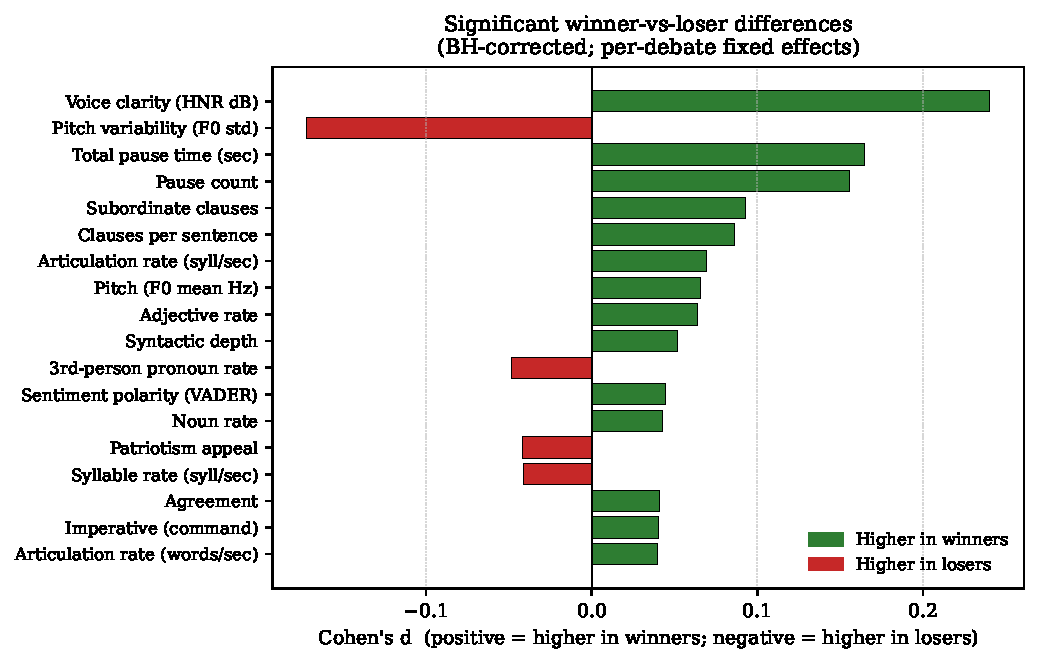
\includegraphics[width=0.95\textwidth]{figures/fig3_effects.pdf}
  \caption{Significant winner-vs-loser differences
  (Benjamini--Hochberg corrected at $\alpha = 0.05$, with per-debate
  fixed effects). Bars show Cohen's $d$; positive (green) bars
  indicate higher in winners; negative (red) bars indicate higher in
  losers. The four largest effects are acoustic; the largest
  text-side effects are on syntactic complexity and patriotism.}
  \label{fig:effects}
\end{figure*}

\subsection{Pause Behavior}
Fig.~\ref{fig:pauses} illustrates the pause distributions. Winners
pause more in both \emph{duration} and \emph{count}, even after
per-debate fixed-effects control. We hypothesize that
deliberate pausing serves as an authority signal in
high-stakes speech.

\begin{figure}[!t]
  \centering
  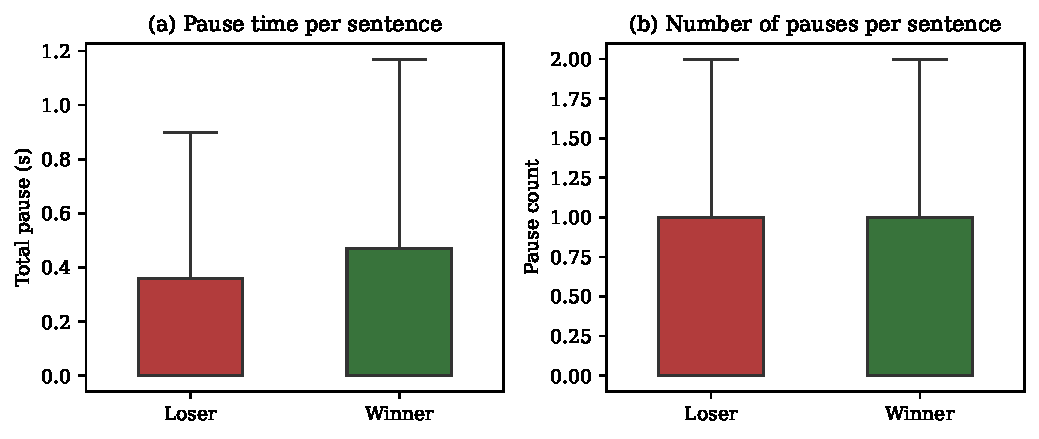
\includegraphics[width=\columnwidth]{figures/fig4_pauses.pdf}
  \caption{Pause distributions per candidate sentence. Boxes show
  IQR; whiskers extend to $1.5\times \text{IQR}$. Outliers omitted
  for visual clarity. Winners consistently take more and longer
  pauses across the corpus.}
  \label{fig:pauses}
\end{figure}

\subsection{LDA Classification on openSMILE Features}
Table~\ref{tab:lda} reports the openSMILE LDA classification accuracy
under three regimes. The leave-one-debate-out result ($0.681$) is the
methodologically appropriate honest estimate. It is well above the
$0.50$ chance baseline ($p < 10^{-20}$, exact binomial against
$0.50$), demonstrating that the winner-vs-loser distinction has a
transferable acoustic signature independent of which candidate is
speaking.

\begin{table}[t]
\caption{LDA on $88$ openSMILE eGeMAPSv02 features
($n = 25{,}648$, classes nearly balanced). Leave-one-debate-out is
the honest estimate.}
\label{tab:lda}
\centering
\begin{tabular}{lr}
\toprule
Evaluation regime                         & Accuracy \\
\midrule
Training (in-sample)                      & $0.772$ \\
$5$-fold stratified CV                    & $0.771 \pm 0.007$ \\
\textbf{Leave-one-debate-out CV}          & $\mathbf{0.681 \pm 0.041}$ \\
Chance baseline                           & $0.500$ \\
\bottomrule
\end{tabular}
\end{table}

Fig.~\ref{fig:lda} visualizes the LDA projection. Winner and loser
distributions overlap but separate cleanly along LD$1$, with winners
shifted toward higher voice clarity, more controlled prosody, and
lower mean loudness. The top discriminating openSMILE features by
absolute LDA weight are:

\begin{enumerate}
  \item \texttt{loudness\_sma3\_amean} ($\beta = -2.03$): losers
        are louder on average.
  \item \texttt{mfcc3V\_sma3nz\_amean} ($\beta = +1.67$): voiced
        spectral-shape pattern higher in winners.
  \item \texttt{spectralFluxV\_sma3nz\_amean} ($\beta = +1.33$):
        winners more spectrally dynamic.
  \item \texttt{F1frequency\_sma3nz\_amean} ($\beta = +1.26$):
        first-formant frequency pattern.
  \item \texttt{F2amplitudeLogRelF0\_sma3nz\_amean} ($\beta = +1.12$):
        second-formant amplitude relative to F0.
\end{enumerate}

\begin{figure*}[!t]
  \centering
  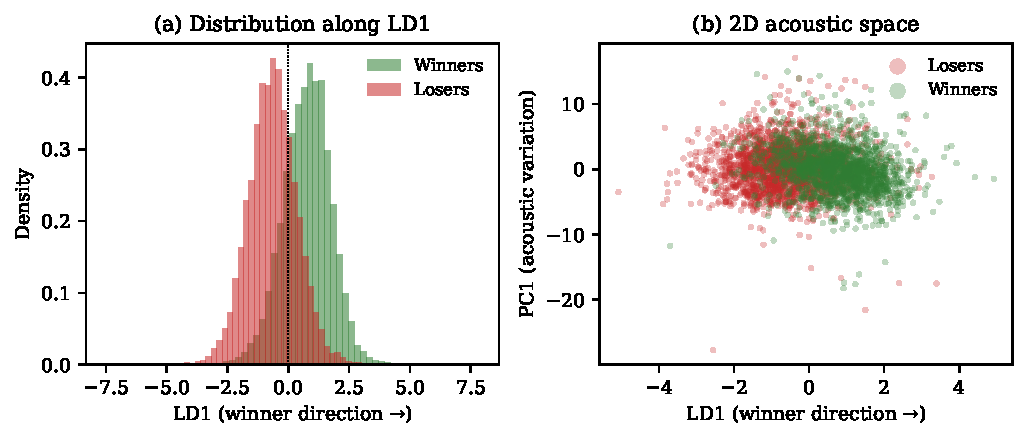
\includegraphics[width=0.95\textwidth]{figures/fig2_lda.pdf}
  \caption{LDA projection of openSMILE eGeMAPSv02 features for
  winner vs.\ loser candidate sentences. (a) $1$D histogram of LD$1$
  scores by class shows substantial separation despite overlap.
  (b) $2$D scatter (LD$1$ vs.\ PC$1$ of the residual space) with
  $4{,}000$-point subsample. Leave-one-debate-out CV accuracy:
  $0.681 \pm 0.041$.}
  \label{fig:lda}
\end{figure*}

\subsection{Temporal and Cross-Era Patterns}
Fig.~\ref{fig:perdebate} reports four key metrics aggregated by
election year. Voice clarity favors winners in nearly every cycle.
Pause-time differences are most pronounced from $1996$ through
$2008$. Sentence length declines sharply post-$2012$, with both
winners and losers adopting clipped speech; the
historical pattern of winners using longer sentences flips in
$2016$.

Table~\ref{tab:decade} provides decade-level sentence-length
statistics. The pre-$2010$ pattern of winners using longer
sentences than losers reverses in the $2020$s. In the $2010$s and
$2020$s, the typical candidate sentence has dropped from
$\sim 15$ words to $\sim 10$ words. We interpret this as a corpus-level
shift in U.S.\ debate rhetoric toward shorter, more attack-oriented
construction in the post-$2016$ era.

\begin{table}[t]
\caption{Mean words per candidate sentence, by decade and result.
The traditional winners-use-longer-sentences pattern reverses in the
$2020$s with the rise of clipped, attack-style speech.}
\label{tab:decade}
\centering
\begin{tabular}{lrrr}
\toprule
Decade & Winner & Loser & W $-$ L \\
\midrule
$1980$s & $14.5$ & $18.2$ & $-3.7$ \\
$1990$s & $17.8$ & $13.6$ & $+4.2$ \\
$2000$s & $14.7$ & $15.2$ & $-0.5$ \\
$2010$s & $13.4$ & $14.6$ & $-1.2$ \\
$2020$s & $10.8$ & $9.7$  & $+1.1$ \\
\bottomrule
\end{tabular}
\end{table}

\begin{figure}[!t]
  \centering
  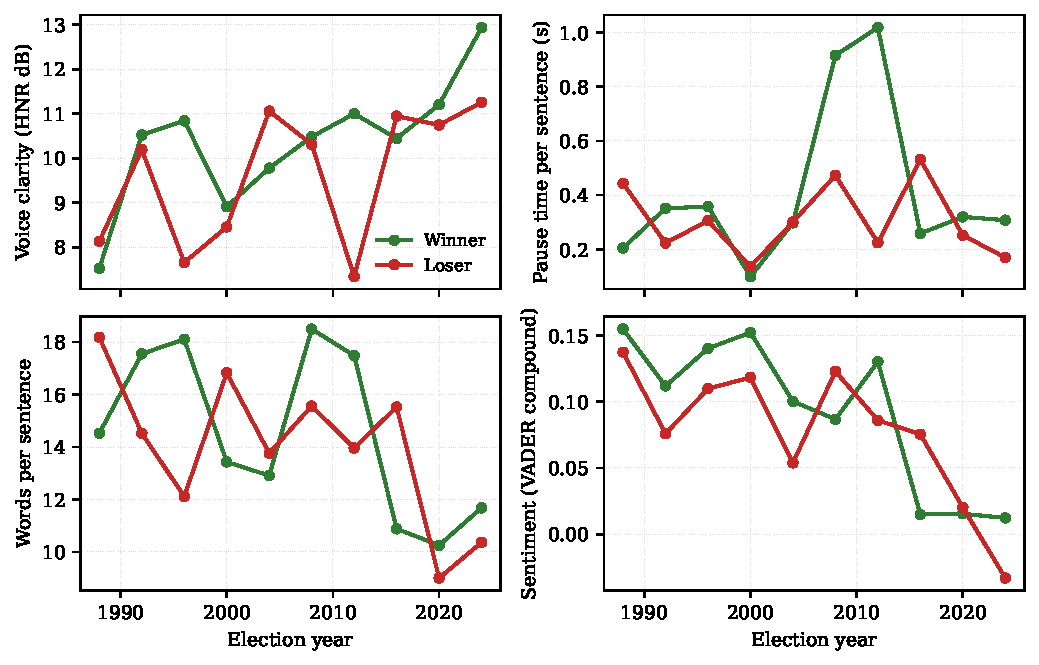
\includegraphics[width=\columnwidth]{figures/fig5_per_debate.pdf}
  \caption{Per-election-cycle trends. Solid green: winners; dashed red:
  losers. Sentence length collapses post-$2012$; voice clarity
  consistently favors winners; pause-time differences are largest
  in the $1996$--$2008$ window.}
  \label{fig:perdebate}
\end{figure}

\subsection{Embedding-Based Semantic Comparison}
Tables~\ref{tab:emb_winner} and \ref{tab:emb_loser} (in
Section~\ref{sec:text}) reported the top-$5$ winner-direction and
loser-direction sentences. Two observations: (i) prototypically
winner-direction sentences cluster around qualified, deliberative
argument with measured concession (``I think it's important for
Governor Romney to present this plan\ldots''); and (ii) sentences
spoken by ultimately-winning candidates can score on the
loser-direction axis when phrased as terse personal attacks
(``You're the worst president America has ever had''). This
indicates that the embedding axis captures \emph{rhetorical register},
not literal class membership---a useful diagnostic property.

\section{Discussion}
\label{sec:discussion}

\subsection{The ``Presidential Bearing'' Pattern}
Across the $26$-debate corpus, a consistent acoustic-rhetorical
pattern emerges. Winners are characterized by:

\begin{itemize}
  \item \textbf{Cleaner phonation} (higher HNR; $d = +0.24$,
        $p < 10^{-173}$).
  \item \textbf{More controlled prosody} (lower F0 std).
  \item \textbf{More rhetorical pausing} ($38\%$ more pause time,
        $33\%$ more pauses per sentence).
  \item \textbf{Slightly lower average loudness} (per LDA weights).
  \item \textbf{Syntactically denser argument} ($12\%$ more
        subordinate clauses, deeper parse trees).
  \item \textbf{More directive language} (imperatives, explanations,
        agreements, rejections all winner-skewed).
\end{itemize}

We interpret these jointly as the technical correlates of the
perceptual quality often described as ``presidential bearing'':
\emph{control}, rather than raw vocal force, is the discriminating
signal. Winners do not yell louder; they speak with more
controlled phonation and give themselves more rhetorical breathing
room.

\subsection{Counter-Intuitive Findings on Patriotism and History}
Three text-side findings run against folk-political intuition:

\begin{itemize}
  \item \textbf{Patriotic appeals} (\texttt{bias\_APAT}) are
        $20\%$ \emph{more} common in losers than winners.
  \item \textbf{Historical references} (\texttt{damsl\_HS}) are
        $44\%$ more common in losers than winners.
  \item \textbf{Emotional appeals} (\texttt{bias\_AE}) are
        $20\%$ more common in losers.
\end{itemize}

A plausible interpretation: losing candidates may rely more heavily on
broad-stroke patriotic and historical framing because they have less
to claim on specific policy or governance. Winners spend their
time on \emph{business, economics, government, and law}
(Empath categories all winner-skewed), which suggests substantive
policy fluency rather than appeal-to-symbol rhetoric.

\subsection{Era Effects: Pre- vs.\ Post-2016}
Sentence length collapses post-$2012$, with both classes converging
toward $\sim 10$-word sentences in the $2020$s. The traditional
winners-use-longer-sentences pattern reverses in $2016$. This is a
real corpus-level shift in U.S.\ debate rhetoric, likely a Trump-era
stylistic effect that has propagated across both Republican and
Democratic speakers. The per-debate fixed-effects analysis
\emph{controls} for this shift; the within-debate winner-vs-loser
acoustic signal remains stable even when the absolute sentence-length
norm changes.

\subsection{Methodological Implications}
The hybrid alignment cascade we developed is itself a contribution.
Real-world political corpora rarely have transcripts that match
audio at the verbatim level required by forced aligners; falling
back to verbatim ASR (Whisper) for paraphrased or non-existent
transcripts, with diarization-recovered speaker labels, made the
$2024$ debates analyzable for the first time. This cascade
generalizes to any multimodal corpus in which transcript fidelity
varies across source eras.

\section{Limitations and Future Work}
\label{sec:limitations}

\begin{enumerate}
  \item \textbf{Interpolated timing for $\sim 10\%$ of Tier-A-equiv
        words.} Per-sentence acoustic features remain reliable because
        they aggregate over many words, but per-word analyses on the
        four text-aligned debates should weight inversely by
        interpolation distance.
  \item \textbf{Winner/loser defined by election outcome.} A complementary
        analysis would use per-debate polling (CNN flash poll, Gallup
        post-debate) as the dependent variable; these labels would be
        orthogonal to ours and could isolate features predictive of
        per-debate persuasion vs.\ overall electoral success.
  \item \textbf{Some candidates appear in many debates.} Trump appears
        in $4$ debates, Obama in $3$, Bill Clinton and G.\ W.\ Bush
        each in $3$. Per-debate fixed effects partially but not fully
        control for this; a hierarchical mixed-effects model with
        random speaker intercepts is a natural extension.
  \item \textbf{Text-untracked bias tags.} Six BEADS-TAGS bias
        categories (gender bias, cognitive bias, gender dismissal,
        issue avoidance, selective evidence, cultural bias) require
        contextual or world-knowledge reasoning beyond rule-based
        detection. These are reserved for human or LLM annotation in
        future work.
  \item \textbf{Single-language corpus.} The pipeline extends naturally to
        non-English political debates, but acoustic norms (F0 ranges,
        speaking-rate baselines) would need recalibration per language.
\end{enumerate}

\section{Conclusion}
\label{sec:conclusion}

We constructed a $35{,}459$-sentence multimodal corpus covering every
U.S.\ general-election presidential debate from $1988$ through $2024$,
using a hybrid three-tier alignment cascade that achieves $100\%$
sentence-level timing coverage across heterogeneous transcript
fidelity. Across this corpus, candidates whose ticket subsequently
won the presidency differ from those who lost in $28$ acoustic,
linguistic, and discourse features that survive per-debate
fixed-effects control and Benjamini--Hochberg correction. The
strongest single discriminator is voice clarity (HNR; Cohen's
$d = +0.24$, $p < 10^{-173}$), with winners exhibiting cleaner
phonation. Winners also pause more, exhibit lower pitch variability,
construct grammatically denser sentences with more subordinate
clauses, and use slightly more positive sentiment. Counter-intuitively,
losers invoke patriotism, fear appeals, and historical references
more often than winners. A linear discriminant analysis on $88$
openSMILE eGeMAPSv02 features alone achieves $0.681 \pm 0.041$
leave-one-debate-out classification accuracy, demonstrating that
``presidential'' speech carries a transferable acoustic signature
independent of any specific candidate. The full feature panel,
per-feature effect sizes, top discriminating sentences, and code are
released for reuse on additional debate corpora and other forms of
high-stakes political discourse.

\section*{Acknowledgments}
The author thanks the open-source maintainers of MFA, Whisper,
pyannote.audio, Praat, openSMILE, spaCy, sentence-transformers, and
Empath, without whose work this analysis would have been impractical.

\bibliographystyle{IEEEtran}
\bibliography{refs}

\end{document}
